\section{Undertaken Research}\label{sec:research}

Experiments:
\begin{itemize}
    \item Varying assimilation period and ensemble size, constant population
    \item Varying assimilation period and population, constant ensemble size
    \item Varying ensemble size and population, constant assimilation period
\end{itemize}

Visualisations:
\begin{itemize}
    \item Heat map of errors for ap vs es, ap vs pop, es vs pop
    \item Snapshot of model with ensemble members linked to relevant states
\end{itemize}

\subsection{Model}\label{sub:method:model}

The above data assimilation scheme will be implemented in conjunction with an
pedestrian agent-based model known as
\texttt{StationSim}\footnote{https://github.com/Urban-Analytics/dust/blob/master/Projects/ABM\_DA/stationsim/stationsim\_model.py}
which aims to simulate pedestrians crossing from one side of the station to the
other.
StationSim has been developed under an object-oriented framework, and as such
both the model and the agent are represented by classes.
The state of each agent comprises of its positions in two-dimensional continuous
space, whilst the state of the model comprises of the collection of all of the
agents in the model.
At each time-step, the model state is evolved by sequentially evolving the
agents.

The model is initialised by passing a number of arguments to the constructor,
including the number of agents in the population and the dimensions of the
rectangular environment.
Upon initialisation, the model generates a population of agents, each of which
are randomly allocated the following:
\begin{itemize}
    \item Entrance through which to enter the environment.
    \item Exit through which to leave the environment.
    \item Speed at which to traverse the environment.
\end{itemize}
As shown in Figure \ref{fig:sample_model_run}, entrances are located on the
left-hand side of the rectangular environment, and exits are located on the
right-hand side of the environment, with each agent seeking to traverse the
environment from their respective entrance to their respective exit.
Where the paths of agents intersect in time and space, crowding occurs.
Faster agents attempt to pass slower agents, at times getting stuck behind them
--- this can be observed in the trails show in Figure \ref{fig:sample_model_run}
at $(x, y) \approx (65, 55)$.

%\begin{figure}[h]
    %\centering
    %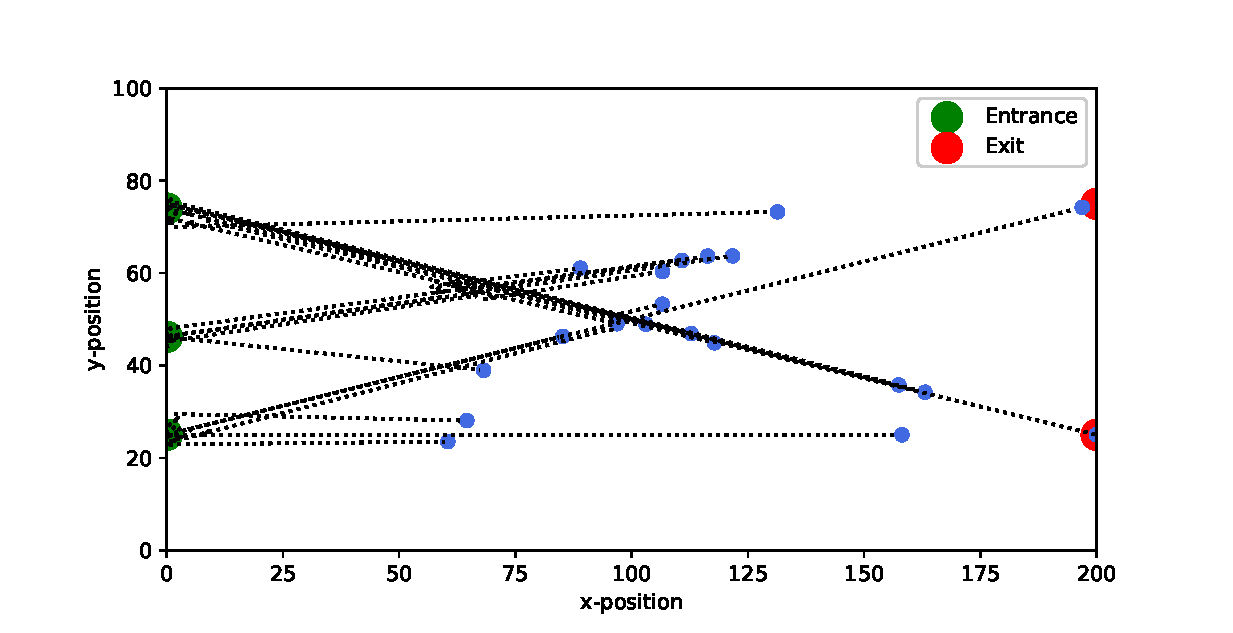
\includegraphics[width=\textwidth]{sample_model_run.eps}
    %\caption{Example run of StationSim for 20 agents; agents enter environment
    %through entrances on left and leave through exits on right.}
    %\label{fig:sample_model_run}
%\end{figure}

\begin{figure}[h]
    \centering
    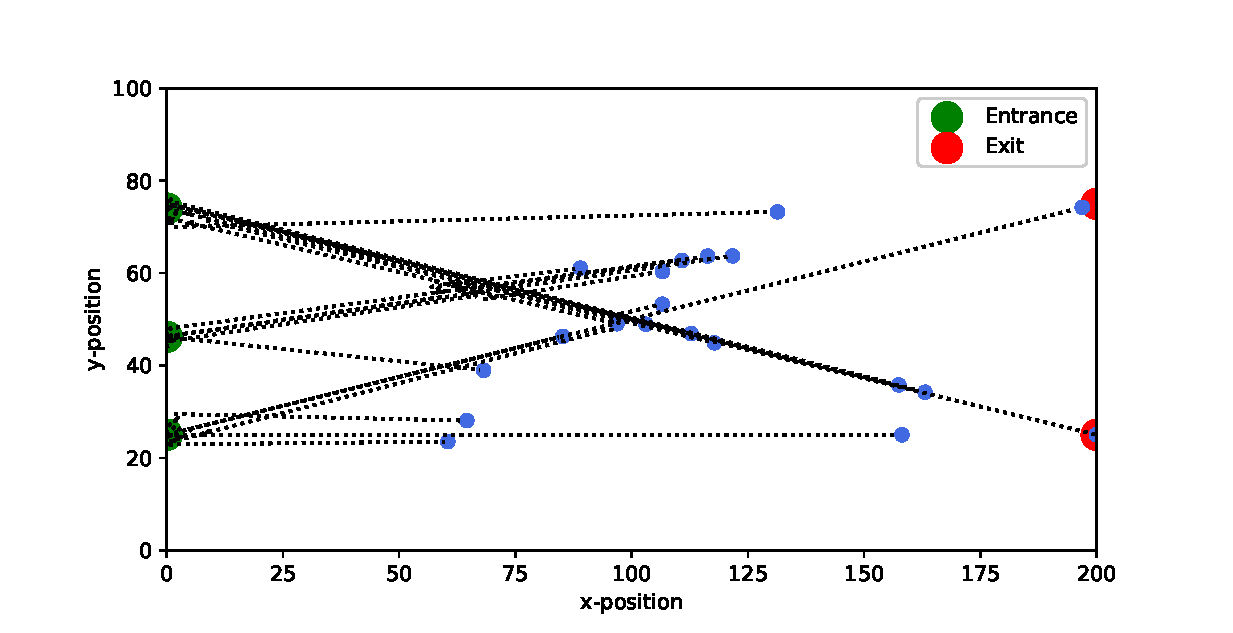
\includegraphics[width=0.8\textwidth]{sample_model_run.eps}
    \caption{Sample model run}\label{fig:sample_model_run}
\end{figure}

\begin{figure}[h]
    \centering
    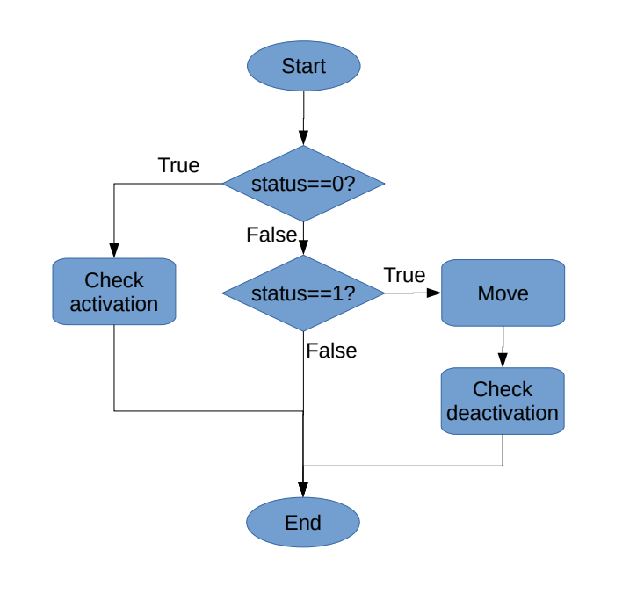
\includegraphics[width=0.8\textwidth]{step.eps}
    \caption{Flow diagram of agent step behaviour. Activation and deactivation
        behaviours are defined in Figure \ref{fig:act_deact}; movement behaviour
    is defined in Figure \ref{fig:move}}\label{fig:step}
\end{figure}

\begin{figure}[h]
    \centering
    \begin{subfigure}[h]{0.4\textwidth}
        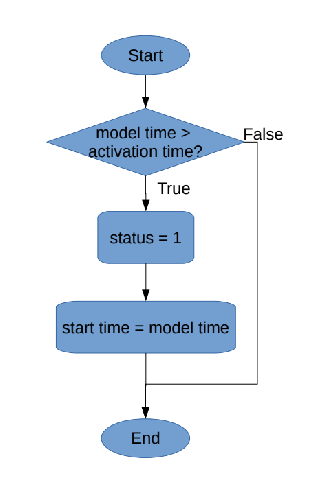
\includegraphics[width=\textwidth]{activate.eps}
        \caption{Activation}\label{fig:act_deact:act}
    \end{subfigure}
    ~
    \begin{subfigure}[h]{0.3\textwidth}
        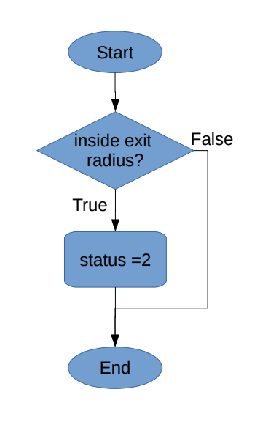
\includegraphics[width=\textwidth]{deactivate.eps}
        \caption{Deactivation}\label{fig:act_deact:deact}
    \end{subfigure}
    \caption{Flow diagrams of agent behaviours for activation and deactivation}
    \label{fig:act_deact}
\end{figure}

%\begin{figure}[h]
    %\centering
    %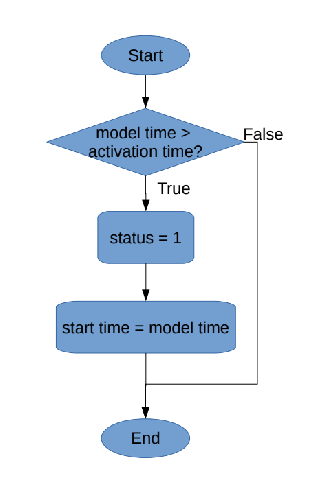
\includegraphics[width=0.5\textwidth]{activate.eps}
    %\caption{Flow diagram of agent step behaviour}
%\end{figure}

%\begin{figure}[h]
    %\centering
    %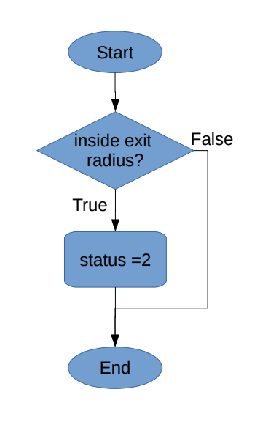
\includegraphics[width=0.5\textwidth]{deactivate.eps}
    %\caption{Flow diagram of agent step behaviour}
%\end{figure}

\begin{figure}[h]
    \centering
    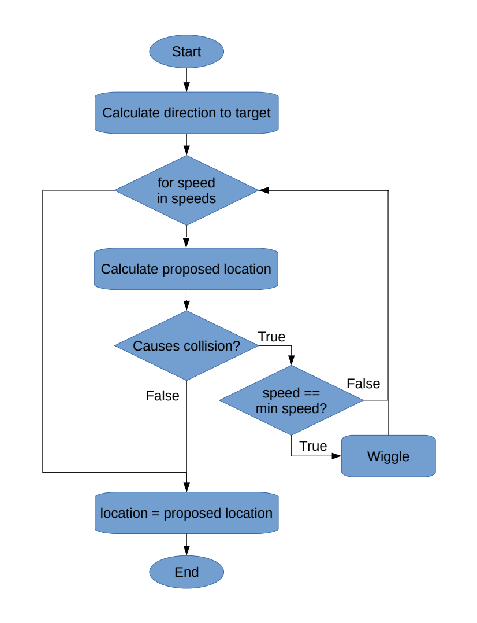
\includegraphics[width=0.8\textwidth]{move.eps}
    \caption{Flow diagram of agent movement behaviour}\label{fig:move}
\end{figure}

\subsection{Experimental Setup}\label{sub:method:experiments}

With the above model in mind, a set of experiments were designed in order to
explore the way in which different factors impact the performance of the
Ensemble Kalman filter when applied to an agent-based model.
In particular, the factors that were explored were:
\begin{itemize}
    \item \textbf{Ensemble Size}: The number of copies of the model that the
        filter maintains.
    \item \textbf{Assimilation Period}: The number of time steps between each
        successive observation being used to update the model states.
    \item \textbf{Measurement Error}: The standard deviation of the noise
        applied to the ground truth data in order to obtain observations.
    \item \textbf{Population Size}: The number of agents created in the model.
\end{itemize}

In order to undertake this investigation, a class was developed in Python to
represent the Ensemble Kalman Filter.
The Python class representing the model is passed to the filter class as an
argument, along with the filter ensemble size, the frequency with which the
filter should assimilate data, and parameters governing the observational noise.
Upon construction, an instance of the filter class creates an instance of the
model, referred to as the \texttt{base\_model}, which takes the parameters given
in Table \ref{tab:model_params}.
Subsequently, an ensemble of models is created by taking deep-copies of the
\texttt{base\_model}, thus ensuring that each of the ensemble members starts
with model- and agent-attributes that match those in the \texttt{base\_model}.

The instance of the filter class steps forward through time according to the
predict-update cycle.
At each predict step, each of the ensemble member models are stepped forward
once, along with the base model; the frequency with which the filter undertakes
the update step is governed by a parameter known as the
\texttt{assimilation\_period}.
Upon reaching the update step of each cycle, the state of each of the ensemble
member models is updated according to equations found in Section
\ref{sec:method:enkf}.
The ground truth for these experiments is taken to be synthetic data generated
by the \texttt{base\_model}; observations are then generated by adding normally
distributed random noise to the ground truth at each assimilation step.

\begin{table}[h]
    \centering
    \begin{tabular}{@{}ll@{}}
        \toprule
        Variable                       & Value                         \\ \midrule
        Number of iterations           & 300                           \\
        Assimilation period            & $[2, 5, 10, 20, 50]$          \\
        Ensemble size                  & $[2, 5, 10, 20, 50]$          \\
        Observation standard deviation & $[0.5, 1.0, 1.5, 2.0, 2.5]$   \\ \bottomrule
    \end{tabular}
    \caption{Table of filter parameters for experiments.}\label{tab:filter_params}
    \label{tab:filter_params}
\end{table}

\begin{table}[h]
    \centering
    \begin{tabular}{@{}ll@{}}
    \toprule
        Variable            & Value                 \\ \midrule
        Population size     & $[5, 10, 15, 20, 25$] \\
        Number of entrances & 3                     \\
        Number of exits     & 2                     \\
        Environment height  & 100                   \\
        Environment width   & 200                   \\ \bottomrule
    \end{tabular}
    \caption{Table of model parameters for experiment.}\label{tab:model_params}
    \label{tab:model_params}
\end{table}

%\subsection{Different Types of Ensemble Kalman Filter}\label{sec:method:types}

%Talk about the different types of EnKF and the implications for ensemble size
%\citep{keller2018comparing}.

%\begin{itemize}
    %\item Damping: counteract filter divergence
    %\item Localisation: reduce the effect of spurious correlations
    %\item Hybrid EnKF: Covariance matrix is made up of the weighted sum of the
        %usual covariance matrix and a separate static covariance matrix that
        %encodes prior underlying knowledge about the system
    %\item Dual EnKF: Split the state vector into state and parameters. At
        %assimilation: update parameters, recalculate forecast, update state
    %\item Normal Score EnKF: Developed to handle non-Gaussian PDFs in EnKF. At
        %assimilation: transform state, parameters and measurements into
        %Z-scores, perform EnKF update based on transformed values, transform
        %back from Z-scores
    %\item Iterative EnKF
%\end{itemize}

As outlined in Chapter \ref{sec:method}, the Ensemble Kalman Filter is a data
assimilation method which aims to approximate the effect of the original Kalman
Filter by representing the state of the model on which it is operating as an
ensemble of state samples.
The aim of applying this ensemble method is to overcome the difficulties
encountered by the original Kalman Filter when being applied to non-linear
models, and when attempting to propagate the state covariance matrix for models
with high dimensionality.
This method has been applied to an agent based model of pedestrian movement
(documented in Section \ref{sub:method:model}) with a view to reducing the error
in the model with respect to the ground truth.
This Section will therefore aim to present the results of the preliminary
experiments undertaken.
This is be achieved by first showing the impact of the filtering process on the
overall model state, then focusing in on a single agent in the model.
Finally a comparison of the model error for before updating, after updating and
the observations used to update will be provided at each of the time-steps in
which assimilation takes place.
It should be noted that this section adopts the common terminology of
``forecast'' to mean the state predicted by the model before updating, and
``analysis'' to mean the state after updating.

